%\documentclass[fleqn,compress,utf8,aspectratio=169,t,handout]{beamer}
\documentclass[fleqn,compress,utf8,aspectratio=169,t]{beamer}

\usetheme{LMU}
\input{recommended-settings}

\usepackage[T1]{fontenc}
\usepackage{lmodern}
\usepackage[english]{babel}
\usepackage{amsmath}
\usepackage{amssymb}
\usepackage{mathtools}
\usepackage{graphicx}
\usepackage{booktabs}
\usepackage{csquotes}
\usepackage{xcolor}
\usepackage{tikz}
\usetikzlibrary{arrows.meta,positioning}

\usepackage[style=authoryear,maxcitenames=2,maxbibnames=4]{biblatex}
\addbibresource{references.bib}

\setbeamersize{text margin left=13pt,text margin right=13pt}
\beamertemplatenavigationsymbolsempty
\setbeamercolor{frametitle}{fg=lmu@green}
\graphicspath{{figures/}{figs/}}

\newcommand{\mainclaim}[1]{%
  {\Large\bfseries #1\par}
}

\newcommand{\quietsource}[1]{%
  \vfill{\scriptsize\color{lmu@lightgray}#1\par}
}

\newcommand{\smallsource}[1]{%
  {\scriptsize\color{lmu@lightgray}#1\par}
}

\newcommand{\keyword}[1]{\textbf{\color{lmu@green}#1}}

\title[Hybrid Modeling]{Hybrid Modeling}
\subtitle{Prediction with a Sense of Input Plausibility}
\author[M. Hein]{Manuel Hein}
\institute[LMU]{LMU Munich\\MA Seminar: Recent Advances in Machine Learning}

\hypersetup{
  pdftitle={Hybrid Modeling},
  pdfauthor={Manuel Hein},
  hidelinks
}

\begin{document}

\maketitle

% Speaker note: Open with the one-sentence promise. The talk is about adding a
% second question to classification: not only "which class?", but also "does the
% input look like the world the model was trained on?"

\section{Core Takeaway}
\begin{frame}
  \vspace{0.65cm}
  \mainclaim{A classifier should answer two questions.}

  \vspace{0.8cm}
  \begin{columns}[T,totalwidth=\textwidth]
    \begin{column}{0.47\textwidth}
      \begin{block}{Prediction}
        \centering
        Which class should this input get?

        \vspace{0.35cm}
        {\Large \(p(y\mid x)\)}
      \end{block}
    \end{column}
    \begin{column}{0.47\textwidth}
      \begin{block}{Plausibility}
        \centering
        Does this input look familiar?

        \vspace{0.35cm}
        {\Large \(p(x)\)}
      \end{block}
    \end{column}
  \end{columns}

  \vspace{0.5cm}
  \centering
  \keyword{Hybrid modeling} puts both questions into one model.
\end{frame}

% Speaker note: Keep this slide almost conversational. The goal is to give the
% audience the mental hook before any technical notation appears.

\section{Why Confidence Is Not Enough}
\begin{frame}
  \mainclaim{A discriminative model always has to choose a class.}

  \vspace{0.25cm}
  \centering
  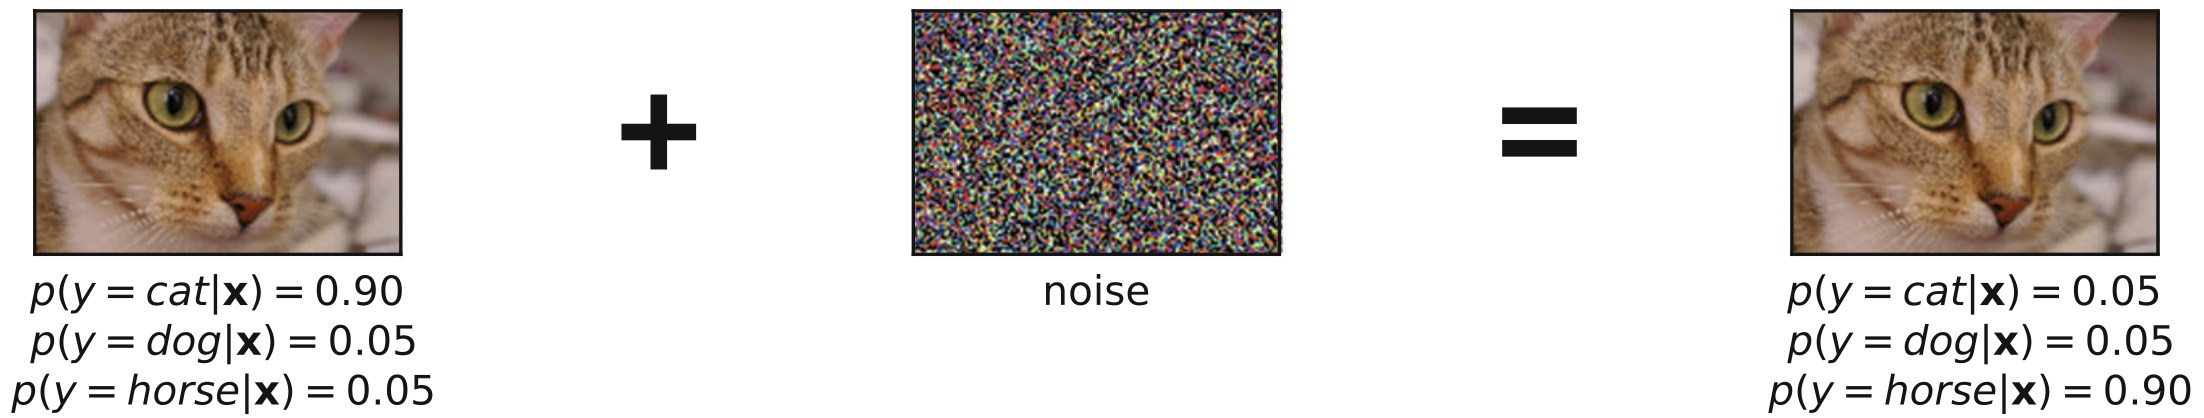
\includegraphics[width=0.96\textwidth]{fig_1_1_confidence_flip.png}

  \vspace{0.2cm}
  \begin{itemize}
    \item High confidence can survive far away from the training distribution.
    \item The missing signal is not another class score, but input plausibility.
  \end{itemize}

  \quietsource{Figure adapted from \textcite{tomczak2024deep}, Fig. 1.1.}
\end{frame}

% Speaker note: Do not overclaim about adversarial examples. Use the image as a
% vivid way to say that class probabilities and familiarity are different ideas.

\section{Discriminative vs Hybrid Thinking}
\begin{frame}
  \mainclaim{The decision boundary is only half of the story.}

  \vspace{0.05cm}
  \centering
  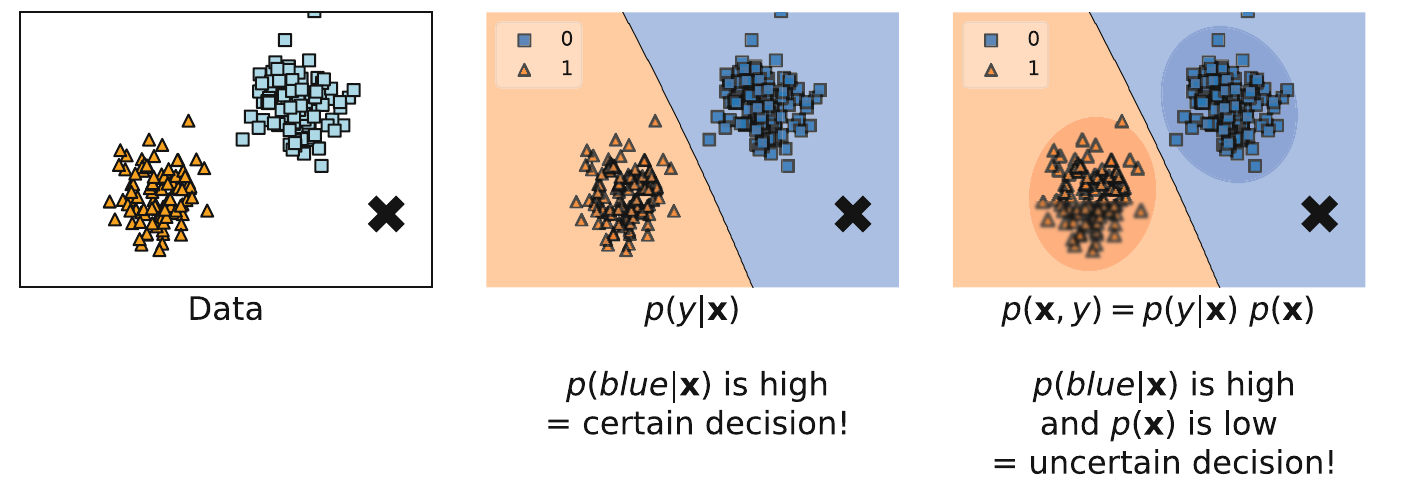
\includegraphics[width=0.76\textwidth]{fig_1_2_discriminative_vs_hybrid.png}

  \vspace{0.12cm}
  \begin{columns}[T,totalwidth=\textwidth]
    \begin{column}{0.48\textwidth}
      \keyword{Discriminative:} choose a side of the boundary.
    \end{column}
    \begin{column}{0.48\textwidth}
      \keyword{Hybrid:} also ask whether the point lies near data.
    \end{column}
  \end{columns}

  \quietsource{Figure adapted from \textcite{tomczak2024deep}, Fig. 1.2.}
\end{frame}

% Speaker note: This is the intuitive bridge to the joint distribution. Mention
% that the hybrid model does not replace classification; it adds the missing view.

\section{The One-Line Idea}
\begin{frame}
  \vspace{0.1cm}
  \mainclaim{Hybrid modeling writes prediction and plausibility together.}

  \vspace{0.35cm}
  \begin{equation*}
    p(x,y)=p(y\mid x)\,p(x)
  \end{equation*}

  \vspace{0.35cm}
  \begin{columns}[T,totalwidth=\textwidth]
    \begin{column}{0.45\textwidth}
      \centering
      \keyword{\(p(y\mid x)\)}\\
      label prediction
    \end{column}
    \begin{column}{0.08\textwidth}
      \centering
      {\Large \(+\)}
    \end{column}
    \begin{column}{0.45\textwidth}
      \centering
      \keyword{\(p(x)\)}\\
      input plausibility
    \end{column}
  \end{columns}

  \vspace{0.35cm}
  \centering
  The goal is \keyword{distribution-aware prediction}, not generation for its own sake.

  \quietsource{\textcite{tomczak2024deep}, Ch. 6.}
\end{frame}

% Speaker note: Say that the equation is simple; the hard part is making both
% terms learn through a useful shared representation.

\section{Flow Recap for This Talk}
\begin{frame}
  \mainclaim{A flow gives us features without throwing the input away.}

  \vspace{0.55cm}
  \begin{columns}[c,totalwidth=\textwidth]
    \begin{column}{0.47\textwidth}
      \begin{itemize}
        \item Map input \(x\) into latent features.
        \item Keep the map invertible.
        \item Evaluate how plausible \(x\) is.
      \end{itemize}
    \end{column}
    \begin{column}{0.47\textwidth}
      \centering
      {\Large
      \[
        z=f^{-1}(x)
      \]
      }
      \vspace{0.1cm}
      \keyword{latent representation}
    \end{column}
  \end{columns}

  \vspace{0.45cm}
  \begin{block}{Only the needed memory jogger}
    A normalizing flow turns a simple latent distribution into a flexible model of data,
    while preserving exact likelihood evaluation.
  \end{block}

  \quietsource{\textcite{tomczak2024deep}, Ch. 4.}
\end{frame}

% Speaker note: The audience has heard about flows, so keep this as a recap. Do
% not derive the Jacobian formula here; say "the correction exists" and move on.

\section{Why Invertibility Matters}
\begin{frame}
  \mainclaim{A classifier can forget details; a density model cannot.}

  \vspace{0.55cm}
  \begin{columns}[T,totalwidth=\textwidth]
    \begin{column}{0.47\textwidth}
      \begin{block}{Classifier features}
        Useful for separating labels.

        \vspace{0.25cm}
        May discard information that is irrelevant for the class.
      \end{block}
    \end{column}
    \begin{column}{0.47\textwidth}
      \begin{block}{Invertible features}
        Useful for prediction.

        \vspace{0.25cm}
        Still retain enough structure to score the input.
      \end{block}
    \end{column}
  \end{columns}

  \vspace{0.65cm}
  \centering
  This makes flows a natural backbone for hybrid modeling.

  \quietsource{\textcite{nalisnick2019hybrid}; \textcite{tomczak2024deep}.}
\end{frame}

% Speaker note: This slide explains why the technical choice is not arbitrary.
% The model needs a representation that is both predictive and probabilistic.

\section{Separate vs Shared Representation}
\begin{frame}
  \mainclaim{Putting two scores next to each other is not yet hybrid learning.}

  \vspace{0.2cm}
  \begin{columns}[T,totalwidth=\textwidth]
    \begin{column}{0.43\textwidth}
      \centering
      \keyword{Separate models}

      \vspace{0.15cm}
      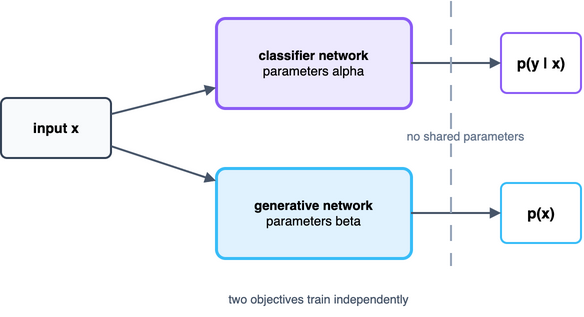
\includegraphics[width=\textwidth]{fig_6_1_naive_separate_models.png}

      \vspace{0.15cm}
      {\small Scores combine, but learning stays separate.}
    \end{column}
    \begin{column}{0.53\textwidth}
      \centering
      \keyword{Shared representation}

      \vspace{0.15cm}
      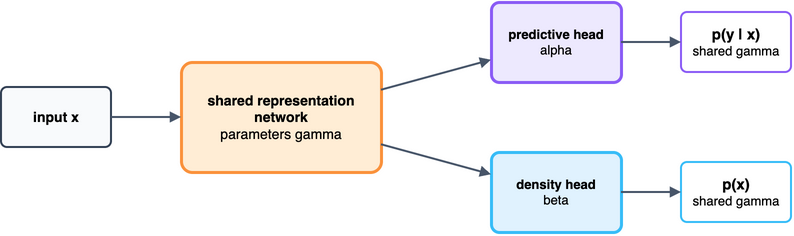
\includegraphics[width=\textwidth]{fig_6_2_shared_parameterization.png}

      \vspace{0.15cm}
      {\small Labels and density shape the same backbone.}
    \end{column}
  \end{columns}

  \quietsource{Figures adapted from \textcite{tomczak2024deep}, Figs. 6.1 and 6.2.}
\end{frame}

% Speaker note: Use this as the first real architecture step. The audience should
% leave with the phrase "shared backbone, two learning signals".

\section{The Scale Mismatch}
\begin{frame}
  \mainclaim{The two learning signals do not arrive at the same volume.}

  \vspace{0.55cm}
  \begin{columns}[T,totalwidth=\textwidth]
    \begin{column}{0.46\textwidth}
      \begin{block}{Label term}
        One class label.

        \vspace{0.25cm}
        A compact supervised signal.
      \end{block}
    \end{column}
    \begin{column}{0.46\textwidth}
      \begin{block}{Input term}
        Many pixels or features.

        \vspace{0.25cm}
        A large density signal.
      \end{block}
    \end{column}
  \end{columns}

  \vspace{0.75cm}
  \centering
  Without balancing, the density objective can pull the shared representation too strongly.

  \quietsource{\textcite{tomczak2024deep}, Sec. 6.2.}
\end{frame}

% Speaker note: Explain the binary example verbally if helpful, but keep the slide
% high-level: one label versus thousands of input dimensions.

\section{The Lambda Dial}
\begin{frame}
  \mainclaim{\(\lambda\) is the practical dial between the two jobs.}

  \vspace{0.35cm}
  \begin{equation*}
    \ell(x,y;\lambda)=\ln p(y\mid x)+\lambda \ln p(x)
  \end{equation*}

  \vspace{0.35cm}
  \begin{columns}[T,totalwidth=\textwidth]
    \begin{column}{0.3\textwidth}
      \centering
      \keyword{small \(\lambda\)}\\
      prediction dominates
    \end{column}
    \begin{column}{0.3\textwidth}
      \centering
      \keyword{balanced}\\
      shared representation
    \end{column}
    \begin{column}{0.3\textwidth}
      \centering
      \keyword{large \(\lambda\)}\\
      density dominates
    \end{column}
  \end{columns}

  \vspace{0.35cm}
  \centering
  Useful, but no longer the cleanest pure likelihood story when \(\lambda\neq 1\).

  \quietsource{\textcite{tomczak2024deep}; \textcite{nalisnick2019hybrid}.}
\end{frame}

% Speaker note: Treat lambda as a dial, not as a theorem. This is the main trade-off
% of the method and should feel memorable.

\section{Hybrid Flow Architecture}
\begin{frame}
  \mainclaim{One invertible backbone does two jobs.}

  \vspace{0.05cm}
  \centering
  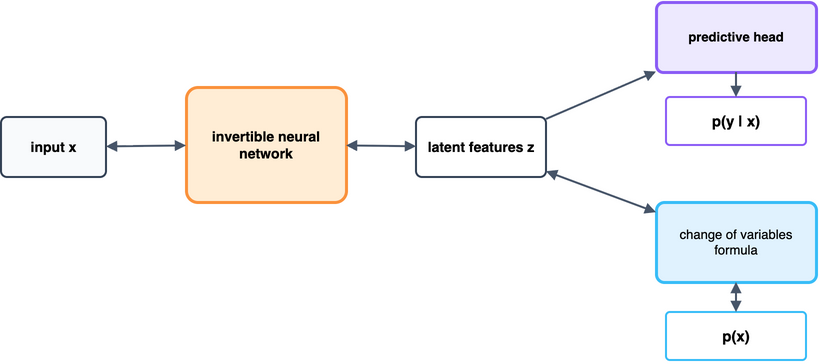
\includegraphics[width=0.64\textwidth]{fig_6_3_hybrid_flow_model.png}

  \vspace{0.08cm}
  \keyword{Predictive head} for labels \hspace{0.7cm}
  \keyword{flow likelihood} for input plausibility

  \smallsource{Figure adapted from \textcite{tomczak2024deep}, Fig. 6.3.}
\end{frame}

% Speaker note: This slide is the architectural summary. Point to the two exits
% from the backbone: prediction and density.

\section{Why HybridIDF Exists}
\begin{frame}
  \mainclaim{Digital images are stored as integers, not as continuous points.}

  \vspace{0.45cm}
  \begin{columns}[T,totalwidth=\textwidth]
    \begin{column}{0.48\textwidth}
      \begin{block}{Continuous flow}
        Natural for real-valued variables.

        \vspace{0.25cm}
        Discrete data often needs dequantization.
      \end{block}
    \end{column}
    \begin{column}{0.48\textwidth}
      \begin{block}{Integer discrete flow}
        Maps integer states to integer states.

        \vspace{0.25cm}
        Probability mass moves without a Jacobian correction.
      \end{block}
    \end{column}
  \end{columns}

  \vspace{0.55cm}
  \centering
  HybridIDF is the hybrid idea adapted to integer-valued data.

  \quietsource{\textcite{hoogeboom2019integer}; \textcite{tomczak2024deep}.}
\end{frame}

% Speaker note: Keep this concrete: 8-bit images have pixel values like 0,...,255.
% IDFs keep the model aligned with that stored representation.

\section{What HybridIDF Shows}
\begin{frame}
  \vspace{0.05cm}
  \centering
  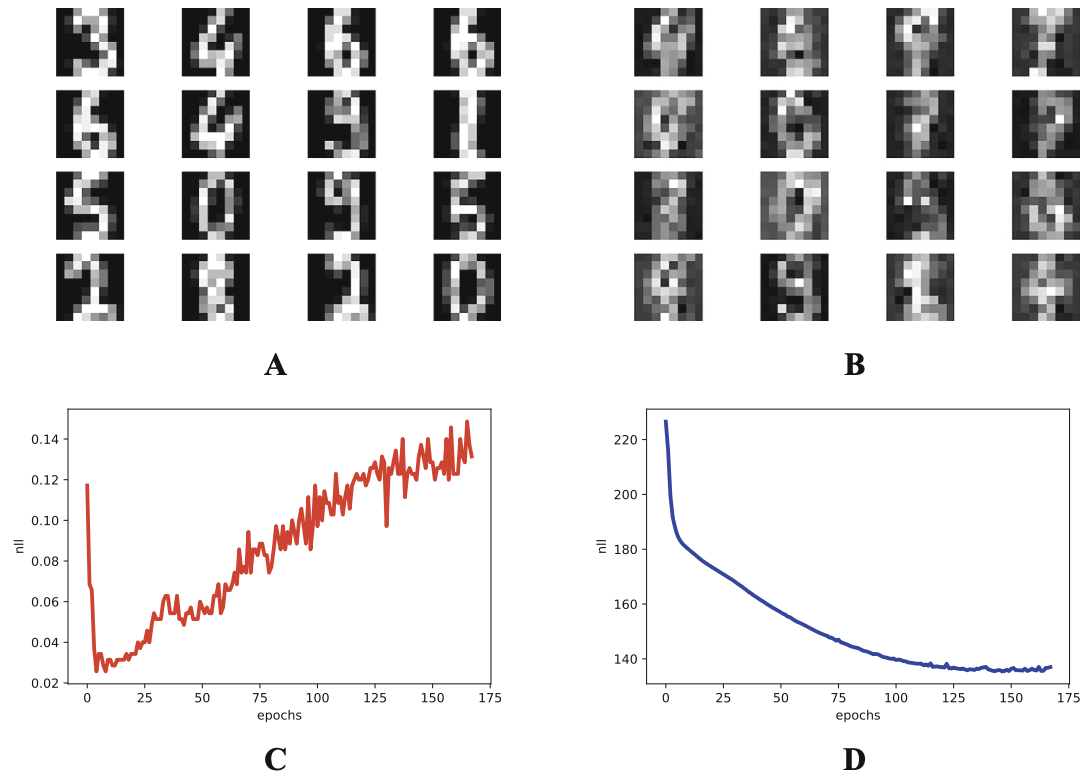
\includegraphics[height=0.62\textheight]{fig_6_4_hybrididf_outcomes.png}

  \smallsource{Figure adapted from \textcite{tomczak2024deep}, Fig. 6.4.}
\end{frame}

% Speaker note: Emphasize that hybrid models need dual evaluation. Do not present
% the figure as a broad benchmark; it is an illustrative trained example.

\section{Benefits and Caveats}
\begin{frame}
  \mainclaim{The extra density view opens doors, but it is not free.}

  \vspace{0.45cm}
  \begin{columns}[T,totalwidth=\textwidth]
    \begin{column}{0.47\textwidth}
      \keyword{What it buys}
      \begin{itemize}
        \item Out-of-distribution signal
        \item Semi-supervised learning route
        \item More informative representations
      \end{itemize}
    \end{column}
    \begin{column}{0.47\textwidth}
      \keyword{What it costs}
      \begin{itemize}
        \item \(\lambda\) must be tuned
        \item Likelihood is not a universal OOD answer
        \item IDFs use biased gradients through rounding
      \end{itemize}
    \end{column}
  \end{columns}

  \quietsource{\textcite{nalisnick2019hybrid}; \textcite{hoogeboom2019integer}; \textcite{tomczak2024deep}.}
\end{frame}

% Speaker note: This is the discussion slide. Keep it honest: hybrid modeling is a
% useful structure, not a magic uncertainty solution.

\section{Final Takeaways}
\begin{frame}
  \vspace{0.45cm}
  \mainclaim{Three things to remember}

  \vspace{0.65cm}
  \begin{enumerate}
    \item Hybrid modeling adds input plausibility to prediction.
    \item Invertible features make the shared representation possible.
    \item The \(\lambda\) dial is powerful, but it is also the central trade-off.
  \end{enumerate}

  \vspace{0.7cm}
  \centering
  A good classifier should know \keyword{what} it sees and whether it has seen something like it before.
\end{frame}

% Speaker note: End with the same sentence family as the opening. This makes the
% talk feel closed instead of like a list of methods.

\appendix

\section{References}
\begin{frame}[allowframebreaks,noframenumbering]
  \printbibliography
\end{frame}

\section{Backup: Equation Chain}
\begin{frame}[noframenumbering]
  \mainclaim{From separate scores to shared learning}

  \vspace{0.25cm}
  \begin{align*}
    \ln p(x,y)
      &= \ln p_\alpha(y\mid x)+\ln p_\beta(x)\\[0.25cm]
    \ln p(x,y)
      &= \ln p_{\alpha,\gamma}(y\mid x)+\ln p_{\beta,\gamma}(x)
  \end{align*}

  \vspace{0.4cm}
  \begin{itemize}
    \item Separate parameters: the two objectives do not shape the same representation.
    \item Shared parameters \(\gamma\): classification and density both update the backbone.
  \end{itemize}

  \quietsource{\textcite{tomczak2024deep}, Eqs. 6.2-6.5.}
\end{frame}

\section{Backup: HybridIDF Objective}
\begin{frame}[noframenumbering]
  \mainclaim{HybridIDF uses discrete probability mass.}

  \vspace{0.15cm}
  \small
  \begin{equation*}
    \ell(x,y;\lambda)
    =
    \sum_{k=1}^{K}[y=k]\ln\theta_{k,g,f}(x)
    +
    \lambda \ln \operatorname{DL}\!\left(z=f^{-1}(x)\mid \mu,\nu\right)
  \end{equation*}
  \normalsize

  \vspace{0.2cm}
  \begin{itemize}
    \item The density term becomes a discretized-logistic mass on integer latents.
    \item Rounded coupling layers keep states integer-valued.
  \end{itemize}

  \smallsource{\textcite{tomczak2024deep}, Eq. 6.13; \textcite{hoogeboom2019integer}.}
\end{frame}

\section{Backup: Empirical Context}
\begin{frame}[noframenumbering]
  \mainclaim{How the supplementary papers support the story}

  \vspace{0.3cm}
  \begin{itemize}
    \item \textcite{nalisnick2019hybrid}: deep invertible features can support exact \(p(x)\) and \(p(y\mid x)\) in one model.
    \item Their experiments used \(p(x)\) as a rejection signal for OOD inputs such as NotMNIST or CIFAR-10.
    \item \textcite{hoogeboom2019integer}: integer discrete flows model ordinal discrete data and support lossless compression.
    \item The report uses these papers as support; the main structure follows \textcite{tomczak2024deep}.
  \end{itemize}
\end{frame}

\end{document}
